\section{Results}
\label{sec:results}

We display the majesty of moosinesq convection in Fig.~\ref{fig:paper_figure02.pdf}.
We visualize the temperature field $T$, so red is warm fluid that buoyantly rises, and blue is cold fluid that buoyantly falls.
Plotted over the temperature field is the mask $\mathcal{M}$, which is fully transparent when it is zero and which is a low-opacity white when $\mathcal{M} = 1$.
This allows us to show that, indeed, there are no appreciable motions outside of the moose and the mask is working properly.

The moose is filled with interesting dynamics\footnote{Likely due to a recent, delicious meal.}.
The legs largely serve as thin, tall ``tunnels'' which are filled with Von K\'{a}rm\'{a}n vortices and which connect the hot moose feet to its neutrally-buoyant body.
Cold fluid parcels from the body have managed to mix down one leg, and the moose would probably benefit from having that leg wrapped in a warm cloth or heat pack.
The body of the moose exhibits dynamics familiar from classical 2D Rayleigh-B\`{e}nard convection.
Hot and cold fluid swirl together, forming many vortices, and mix.
Aside from the legs, the antlers are probably the most interesting part of the moose.
Long-lived vortices of relatively hot fluid establish themselves there and turn for a few convective overturn times.
Then, violent flows from the moose's body disrupt those vortices with fresh, hot fluid and this process repeats itself.
Occasionally some of this hot fluid rises into the tips of the moose's antlers, which probably accounts for the growth of the moose's antlers.

\begin{figure*}[tp!]
\centering
    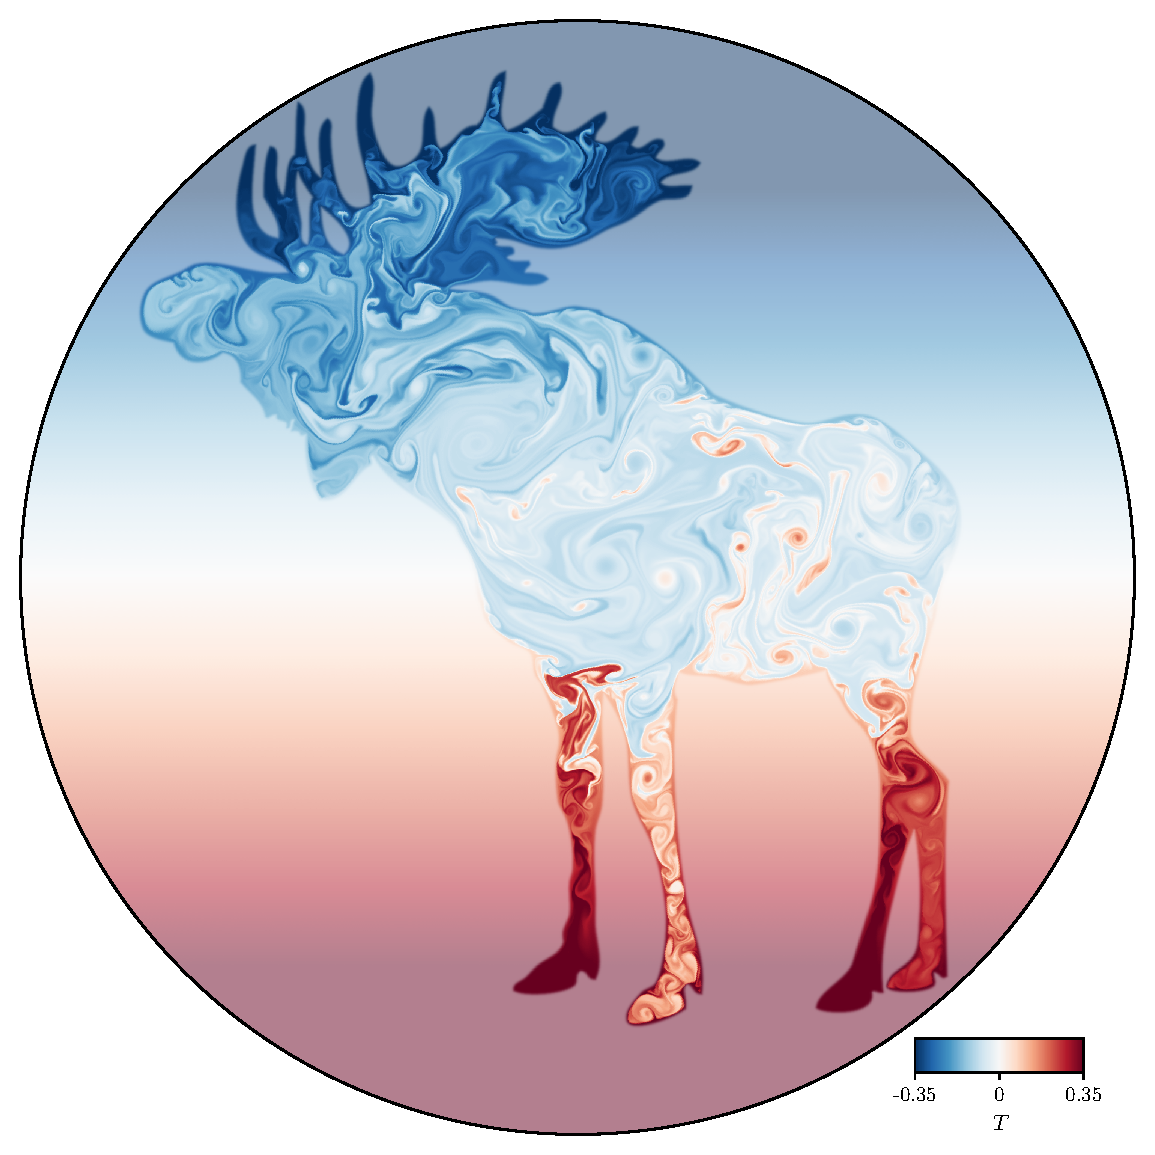
\includegraphics[width=\textwidth]{paper_figure02.pdf}
\caption{ The beautiful, powerful moose.
\label{fig:dynamics}
}
\end{figure*}

Now that we have examined the dynamics in Moosinesq Convection in some detail, we turn our attention towards its astrophysical applications.
\citet{kaiser_etal_2020} note that ``massive [sic] stars'' are sensitive to ``the details of their complex convective history'' \citep{kaiser_etal_2020}.
We agree.
One consideration that previous authors have ignored when considering convective uncertainties in moosive stars is displayed in Fig.~\ref{fig:moosive_stars}.
That is, the cores of these stars are filled with Moosinesq Convection, which can have important consequences for moosive stellar evolution.
it is unclear at this time how the complex flow morphologies associated with moosinesq convection would affect e.g., the magnetic fields, chemical profiles, and lifetimes of these stars.
We leave these important considerations to future work.

\begin{figure*}[t!]
\centering
    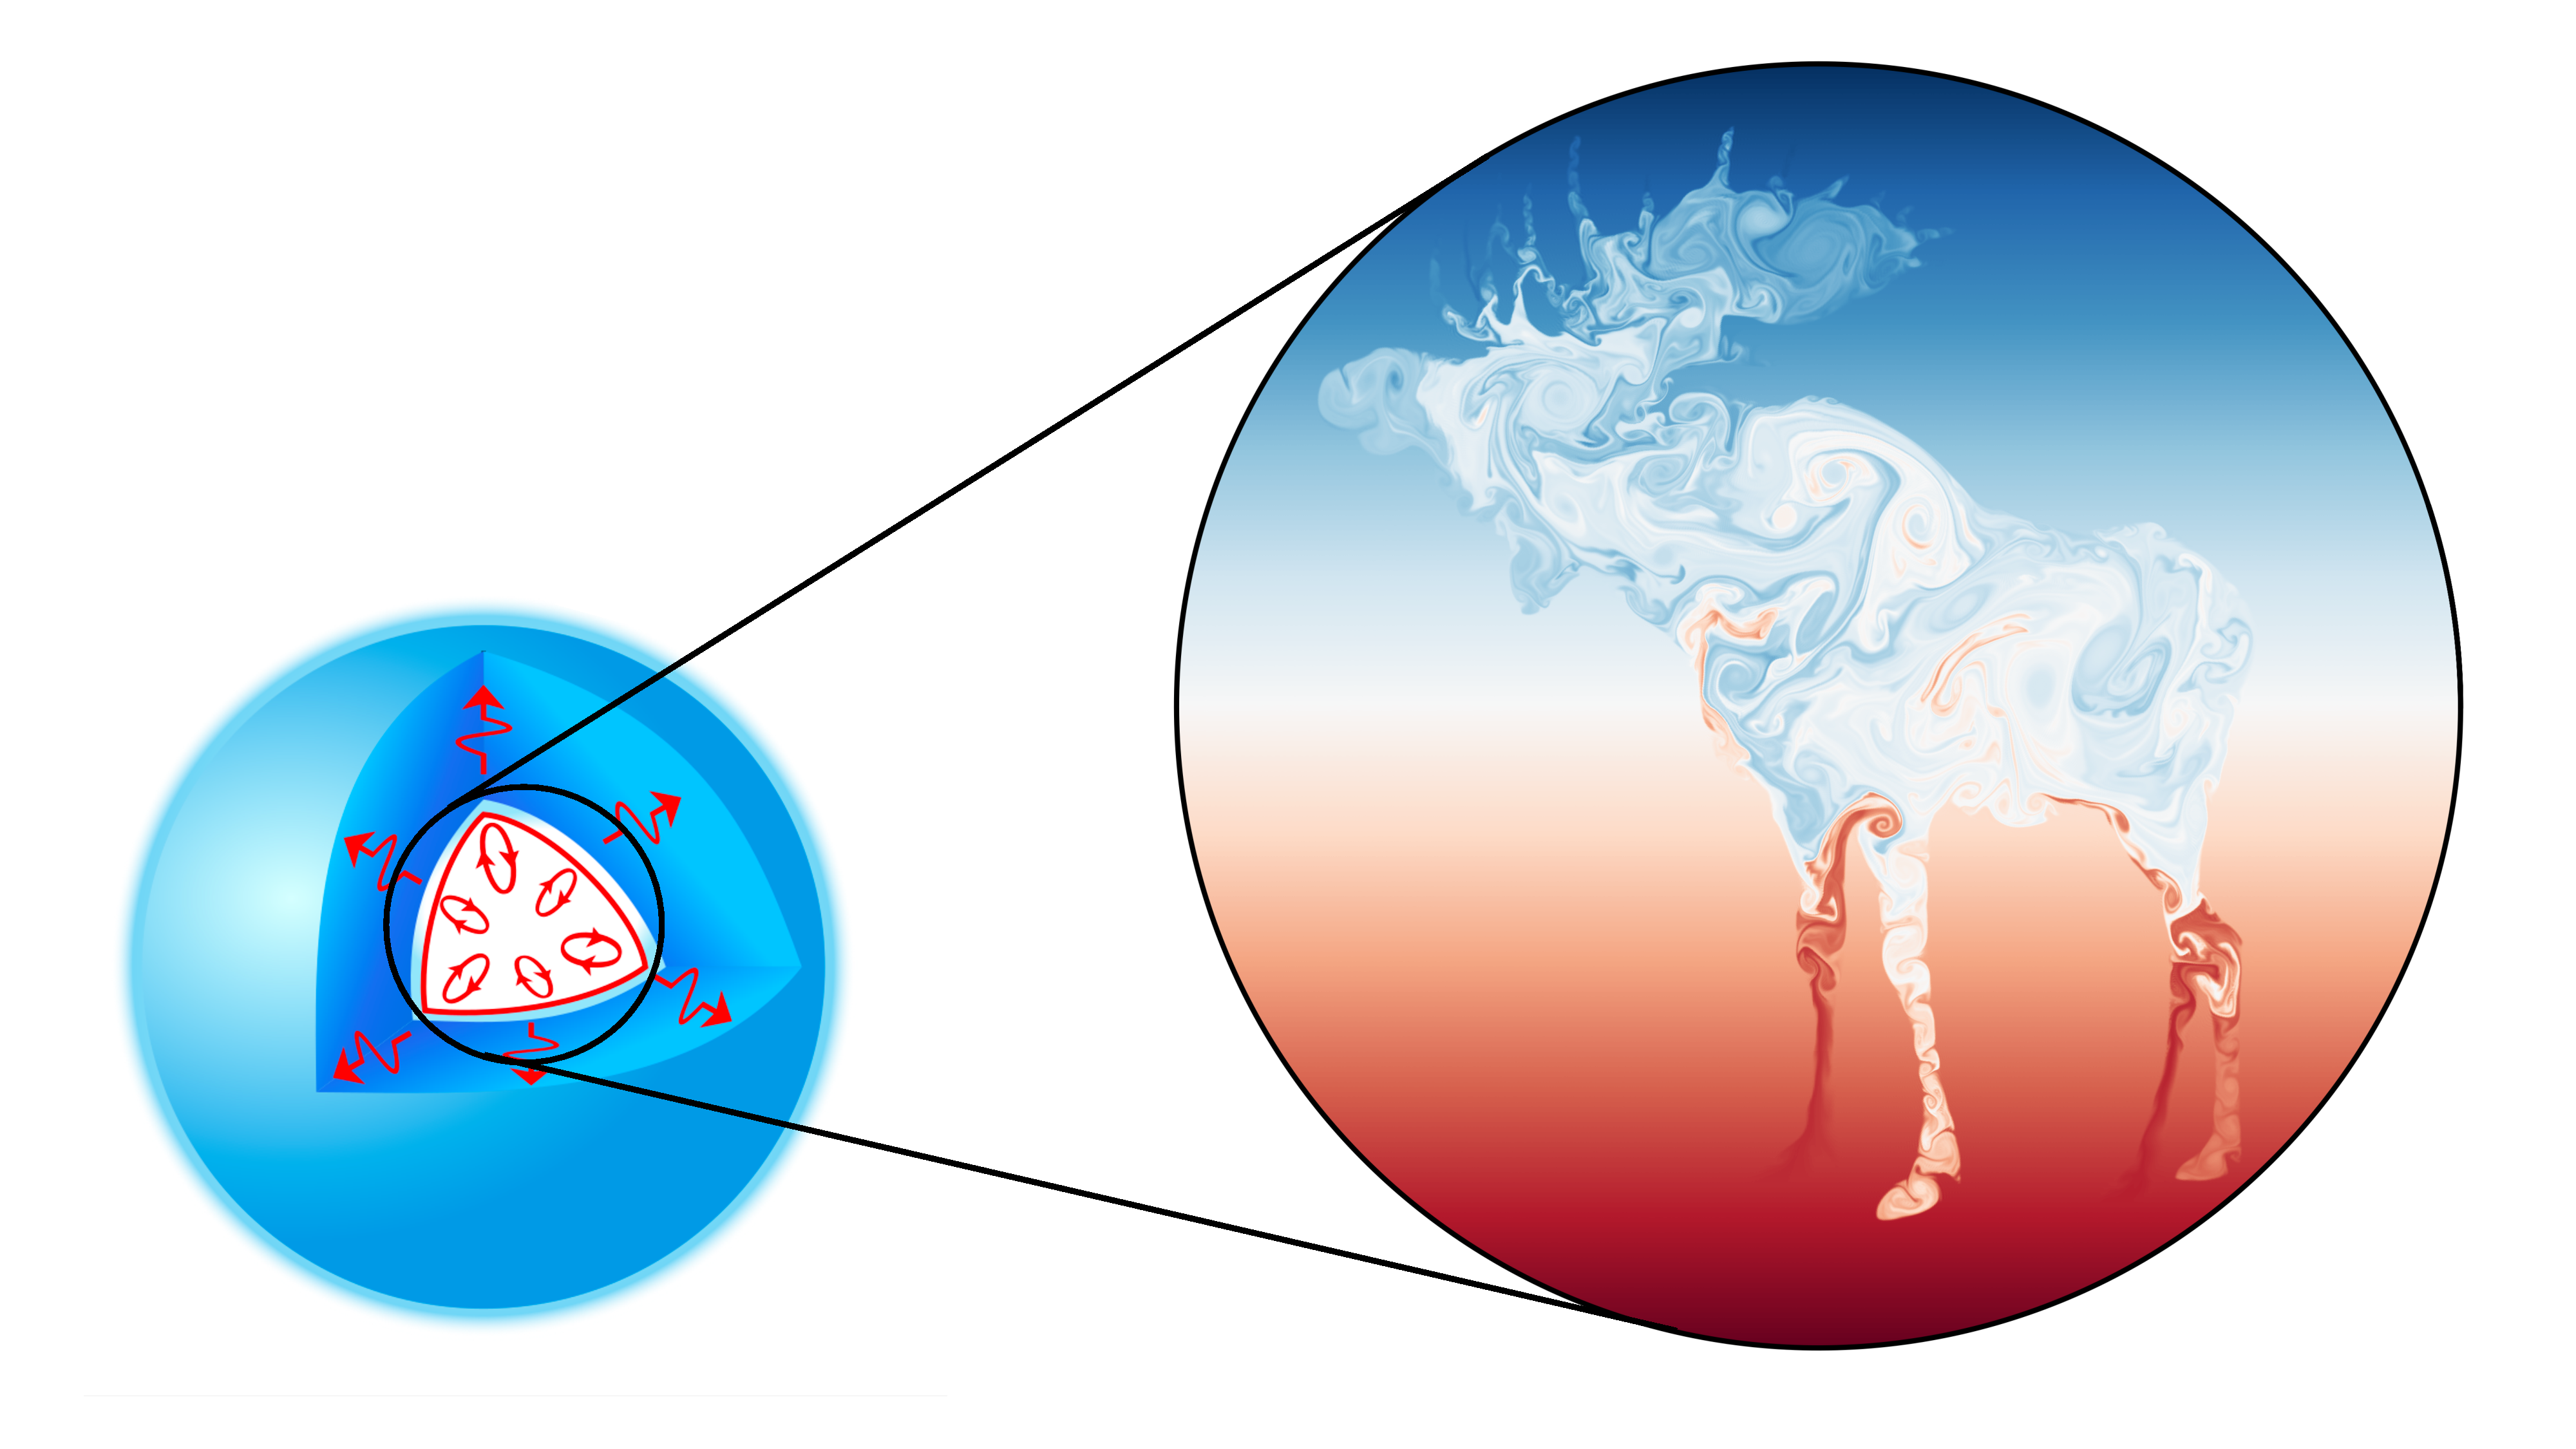
\includegraphics[width=\textwidth]{moosive_stars.pdf}
\caption{ Moosive Stars.
\label{fig:moosive_stars}
}
\end{figure*}


